\chapter{Clase 6. Exposición}
\textbf{25/02/2025}

Cada equipo expuso una solución al problema planteado la clase anterior, el cual era hallar una fórmula para calcular el volumen del prisma grande, y así obtener cuantos prismas pequeños cabían.

\section{Solución 1}
Uno de los equipos expuso de manera geométrica la relación que guardaba cada dobles en la realización de los prismas. Lo que hicieron fue triangular la hoja y observaron qué relación de proporcionalidad se conservaba a medida que se realizaban dobleces en la hoja, aunque en ningún momento llegaron a la solución para conocer la cantidad de prismas pequeños que caben en el prisma grande

\begin{center}
    \begin{figure}[H]
        \begin{tabular}{ccc}    
            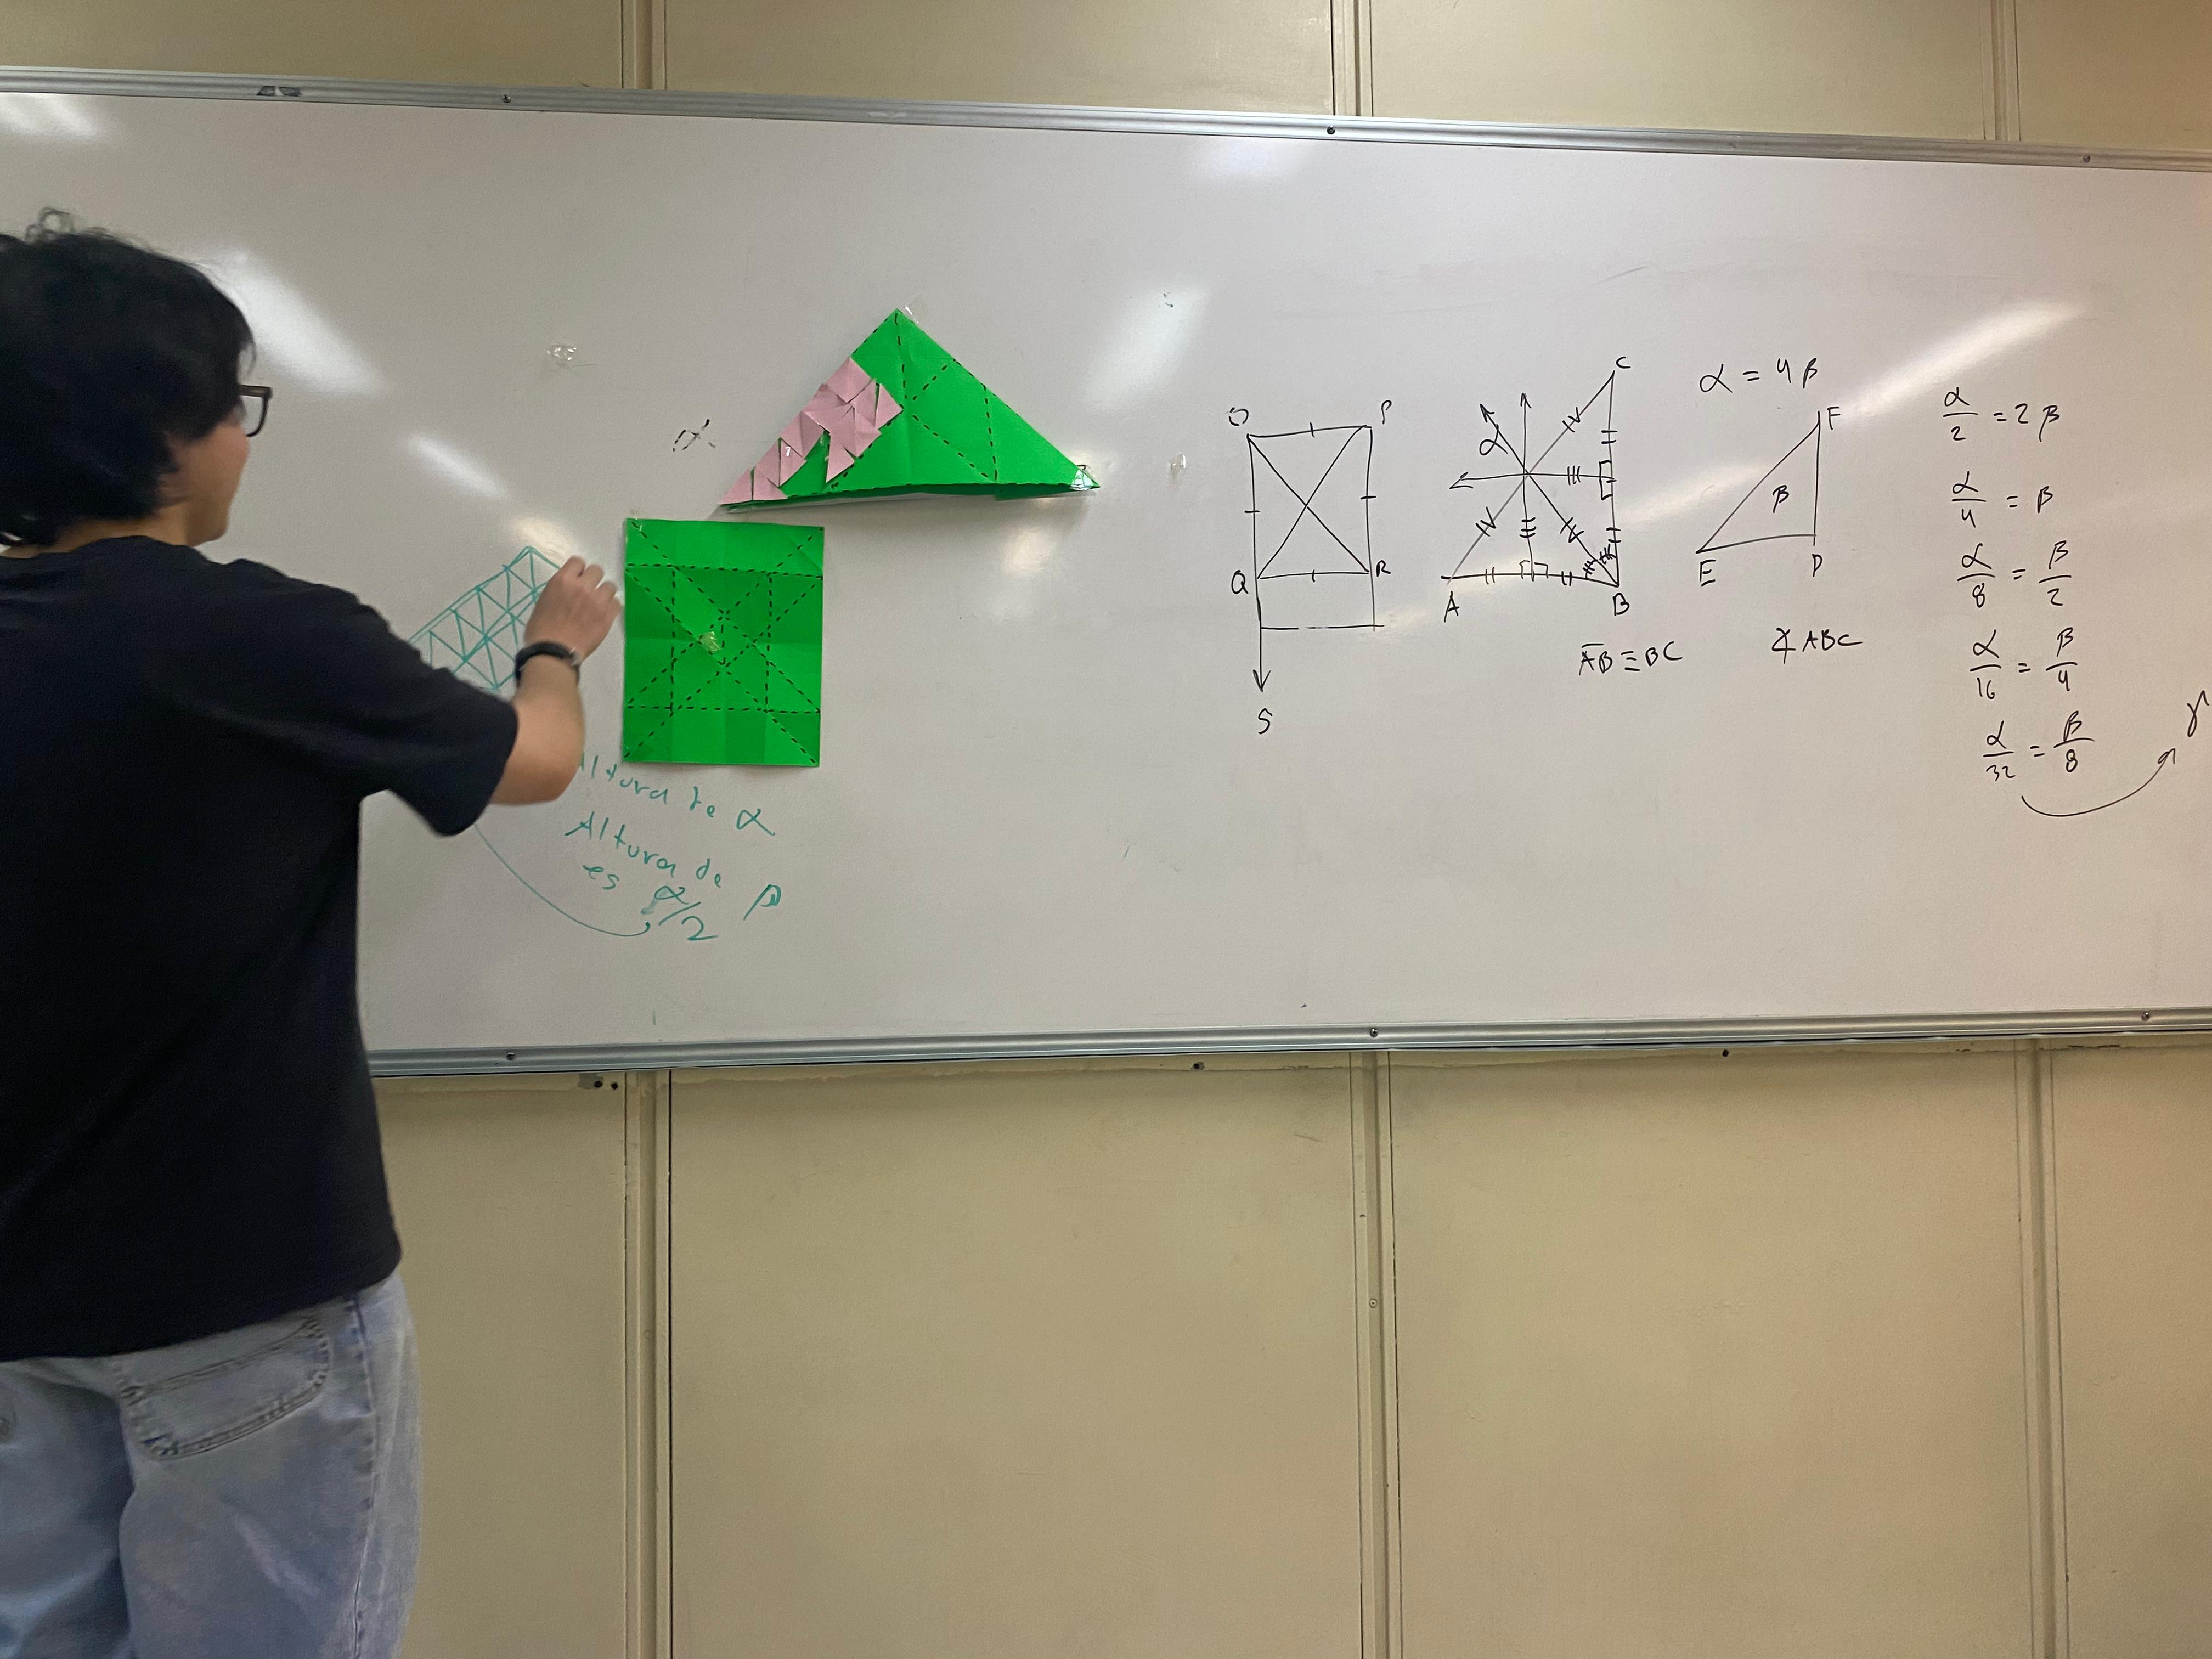
\includegraphics[scale = 0.05]{clase6/Equipo1-1.jpeg}&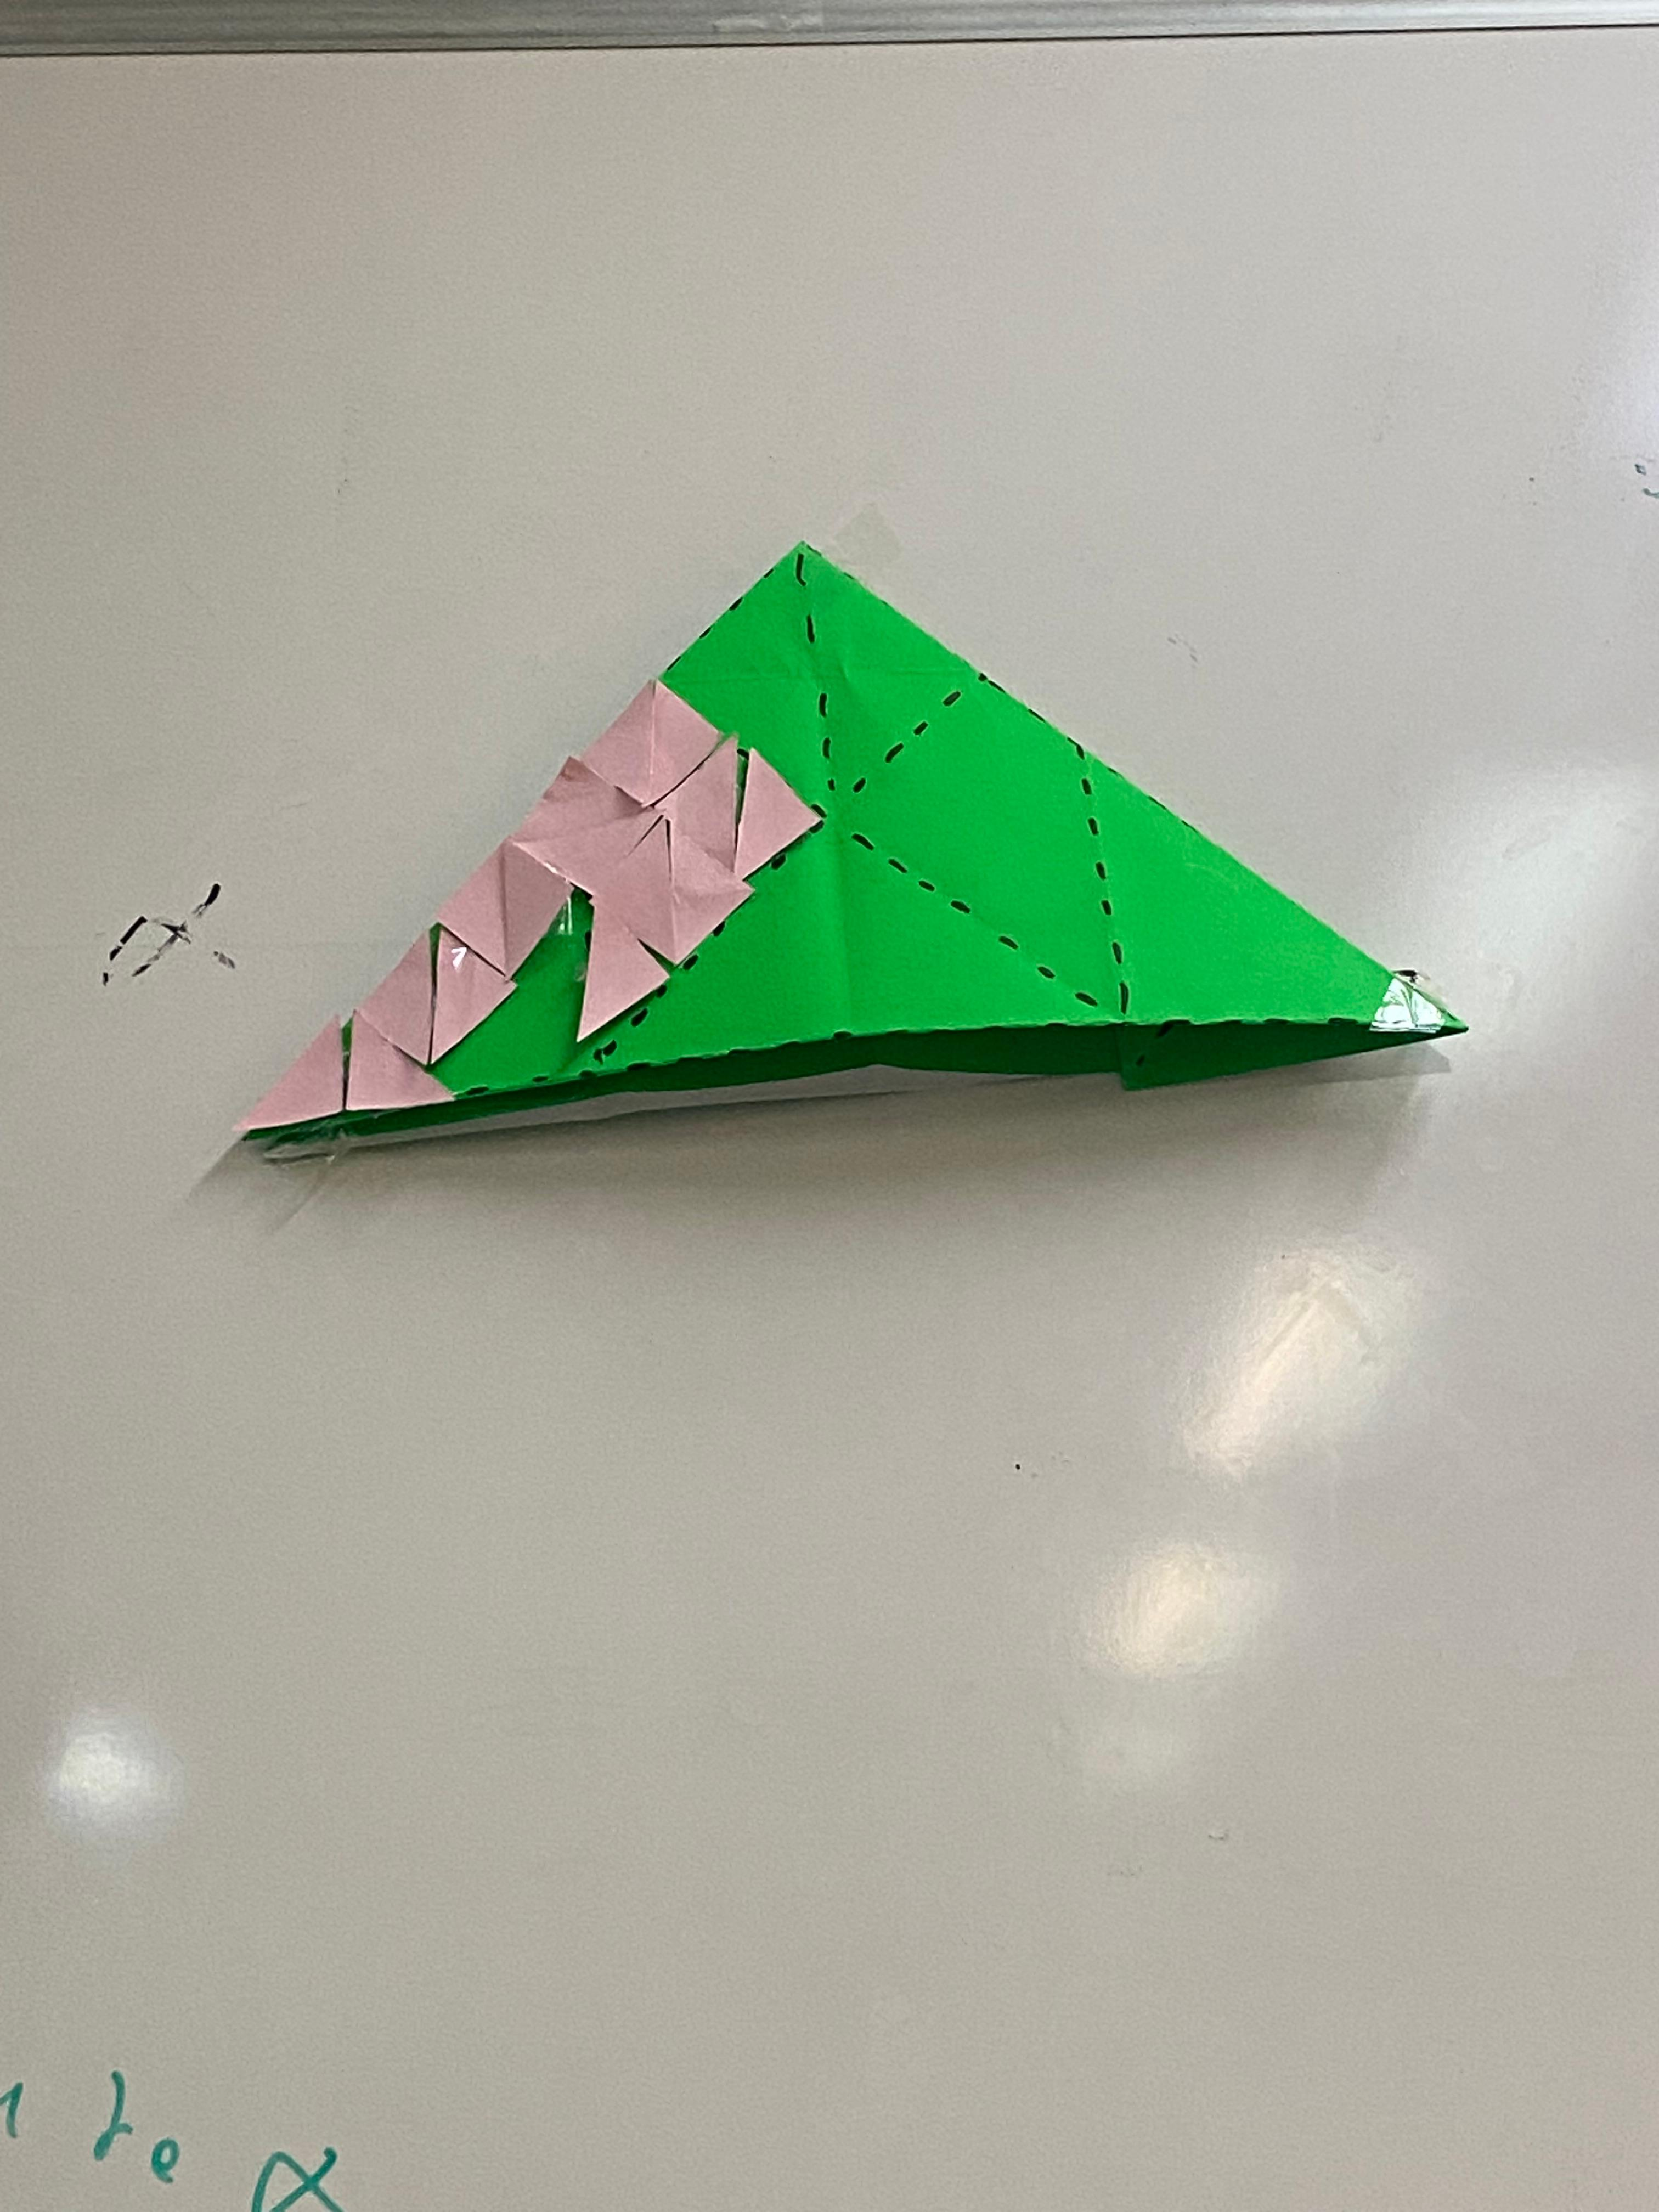
\includegraphics[scale = 0.04]{clase6/Equipo1-2.jpeg}&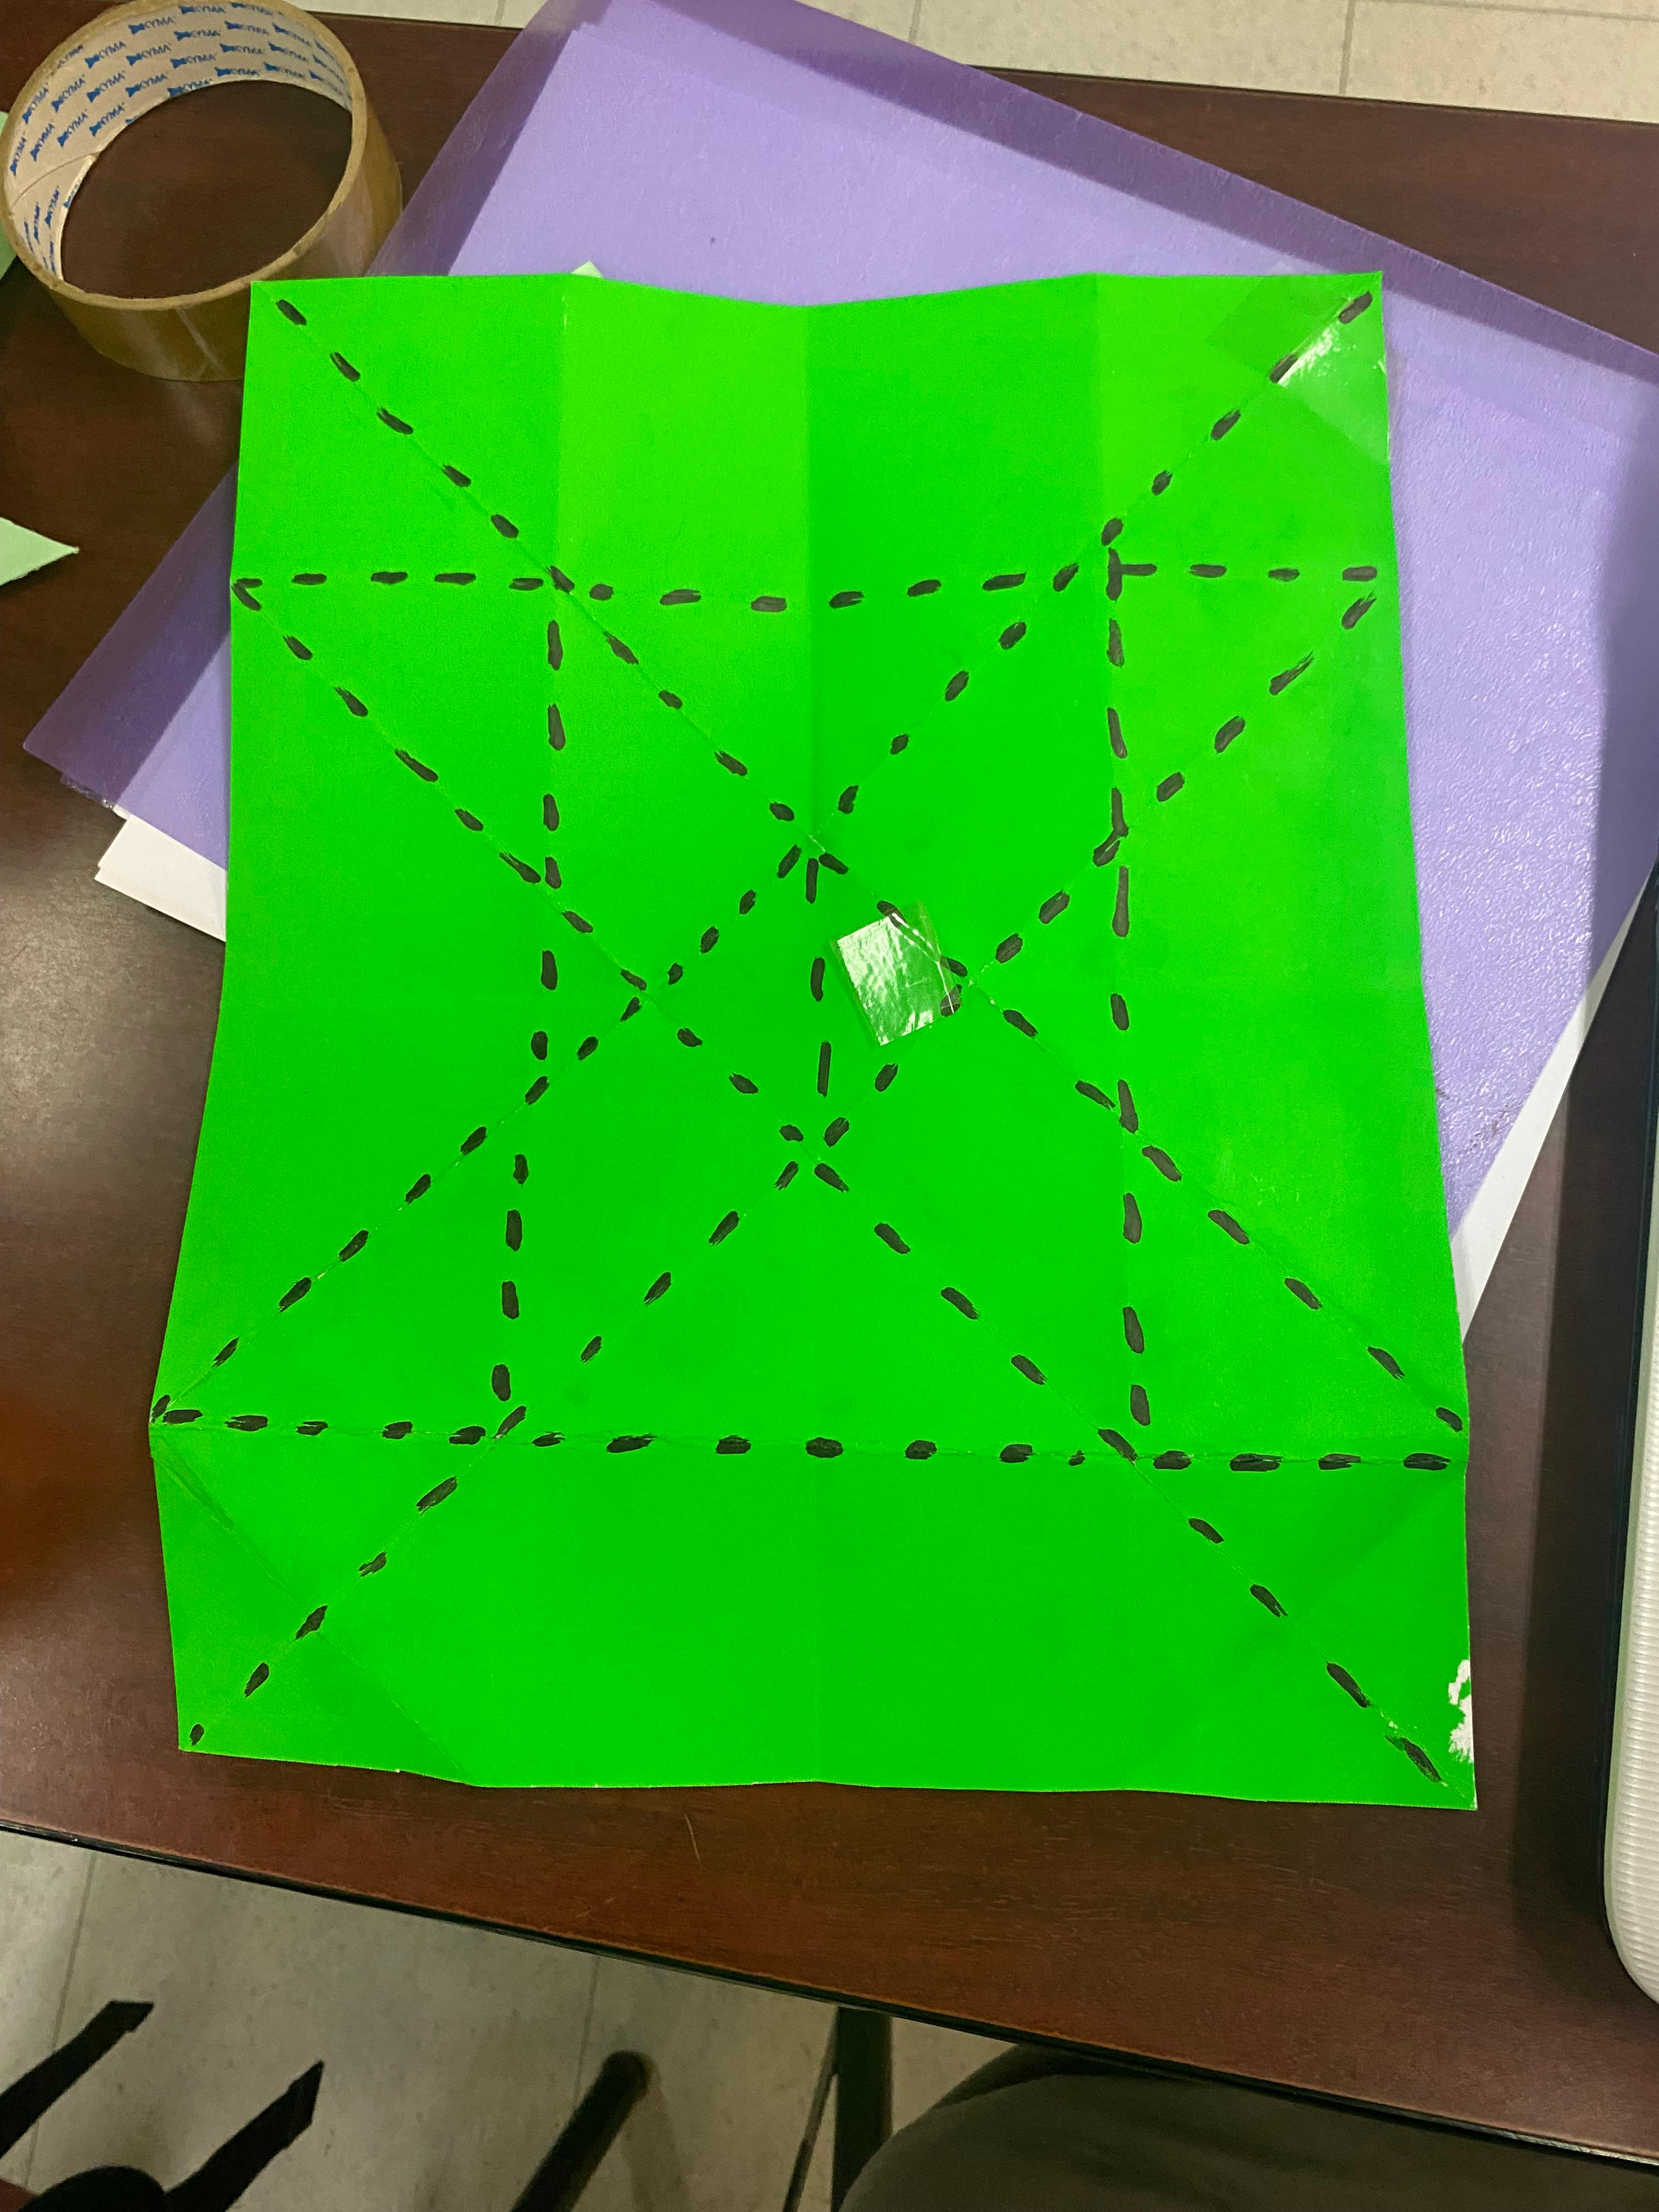
\includegraphics[scale = 0.04]{clase6/Equipo1-3.jpeg}
        \end{tabular}
        \caption{Desarrollo de la solución del equipo 1}
    \end{figure}
\end{center}

\section{Solución 2}

Los equipos restantes y mi equipo tuvimos una idea similar al momento de demostrar de donde obtuvimos la fórmula para calcular el volumen, la cual fue observando que la hoja al momento de ser dividida en cuatro partes, las dimensiones de largo y alto se partían a a la mitad, y aunque no podemos demostrar explícitamente como de una figura en dos dimensiones la medida que nos da la tercera dimensión. Guarda la misma relación. Nuestro argumento fue que al salir el cuerpo geométrico de una figura geométrica (de 2D a 3D), la tercera dimensión iba a guardar la misma relación que las otras dos; consulte \hyperref[chap:C5]{el capitulo anterior para ver el procedimiento que siguió mi equipo.}

\begin{figure}[H]
    \centering %Centra horizontalmente
    \begin{tabular}{cc}
        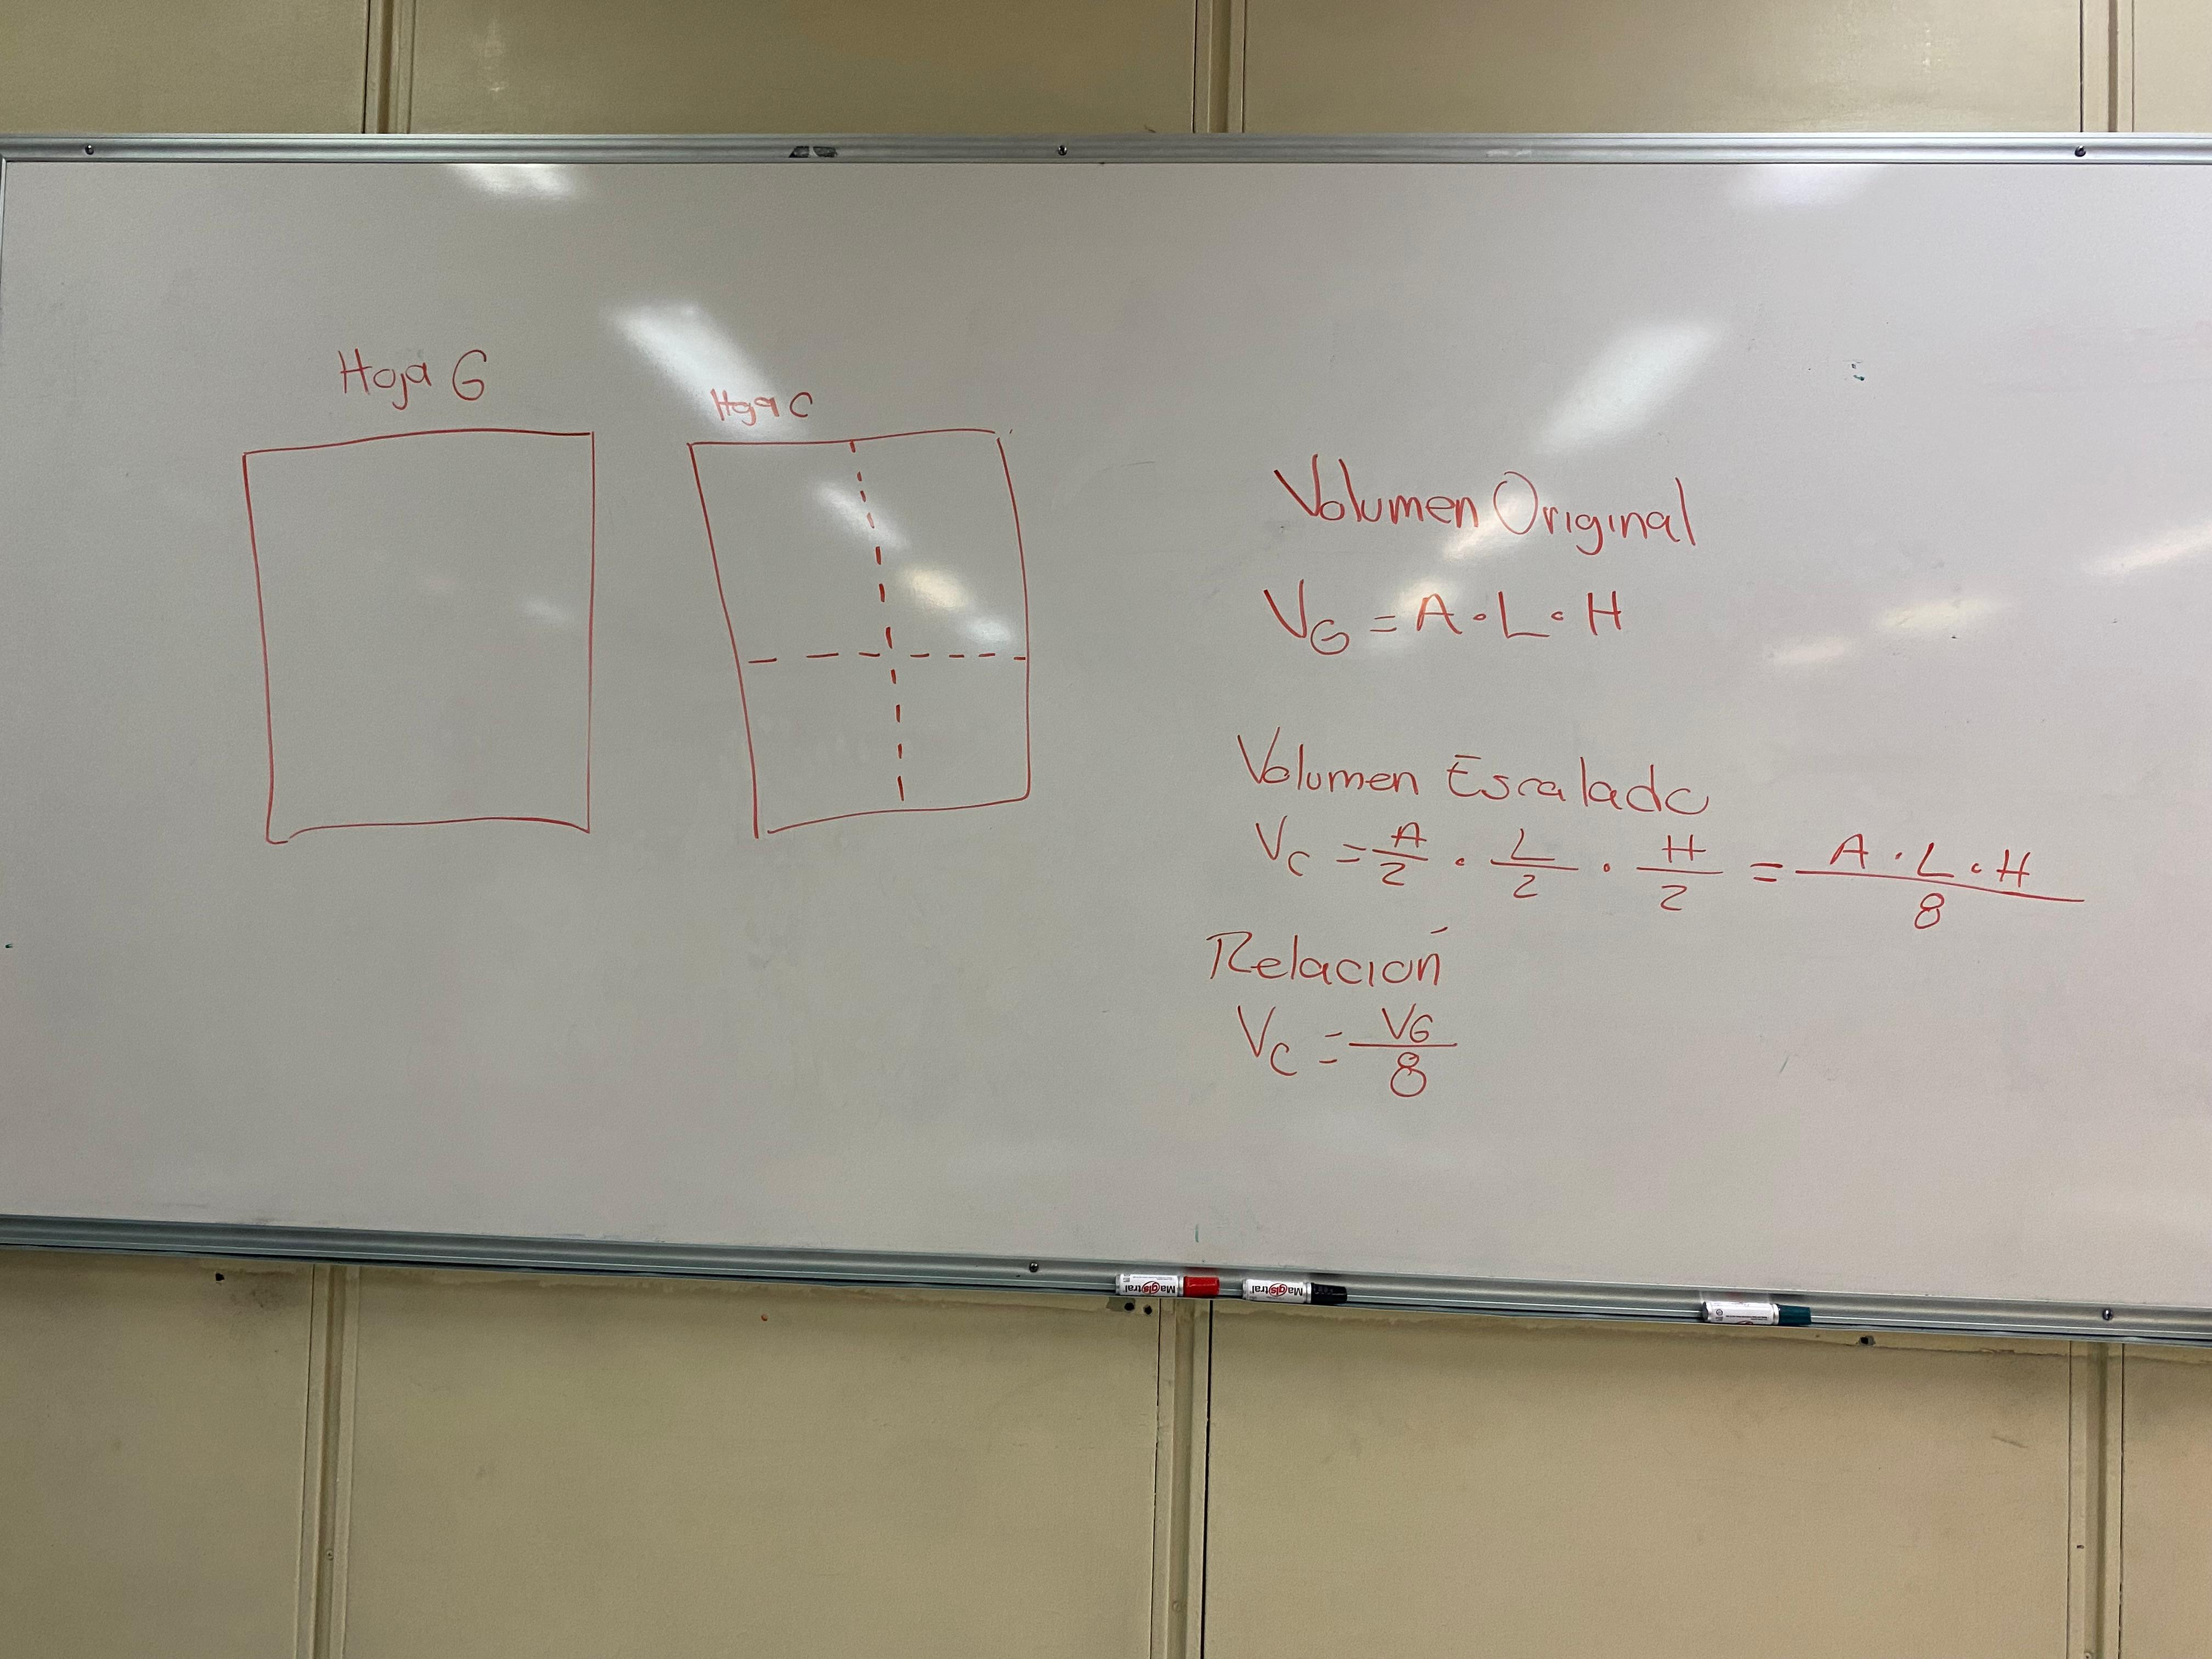
\includegraphics[scale=0.045]{clase6/Equipo2.jpeg}&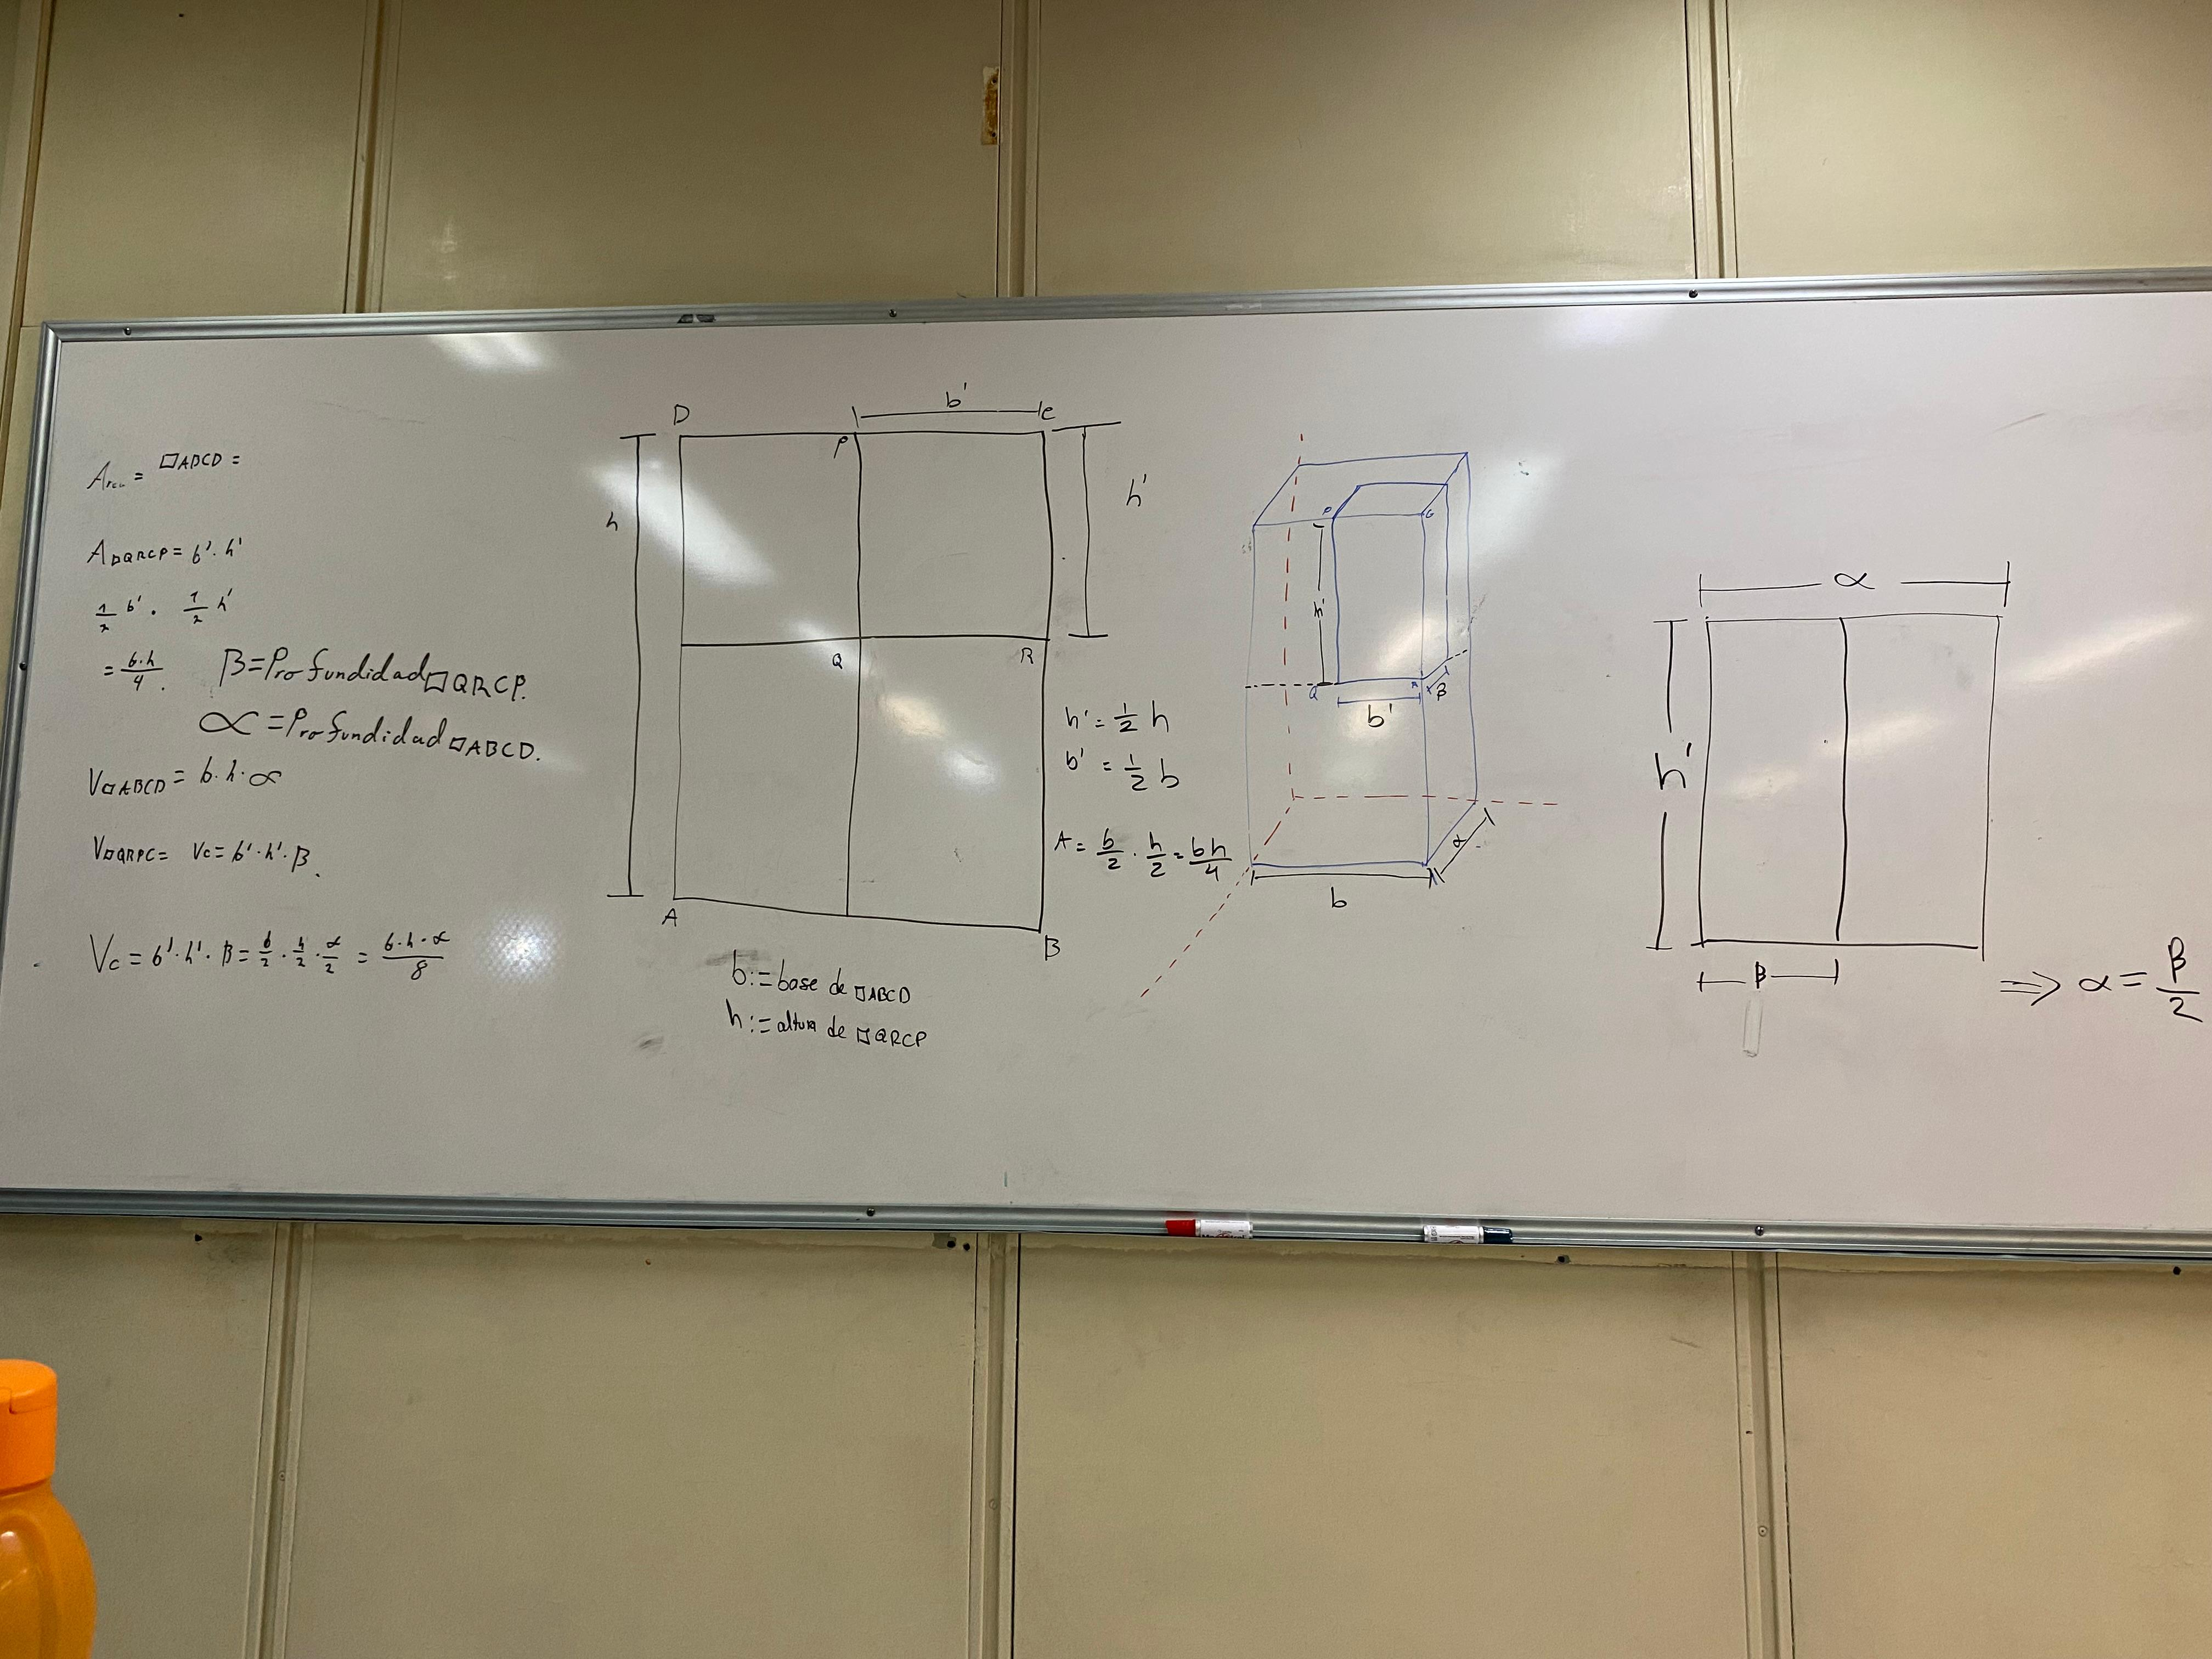
\includegraphics[scale=0.045]{clase6/Equipo3.jpeg}
    \end{tabular}
    \caption{Soluciones similares de los equipos 2, 3 y 4}
\end{figure}